\documentclass[border=4pt]{standalone}
\usepackage[T1]{fontenc}
\usepackage{lmodern}
\usepackage{amsmath}
\usepackage{pgfplots}
\pgfplotsset{compat=1.18}
\usepgfplotslibrary{groupplots,fillbetween}
\usetikzlibrary{calc,arrows.meta}
% one colour per kind of method, the same in every figure (Okabe-Ito)
\definecolor{neur}{HTML}{D55E00}   % neurons chosen by attribution
\definecolor{dirc}{HTML}{009E73}   % directions from the weird-vs-normal contrast
\definecolor{read}{HTML}{0072B2}   % readout methods and interventions chosen from readouts
\definecolor{pers}{HTML}{CC79A7}   % Assistant Axis / persona
\definecolor{ctrl}{HTML}{8C8C8C}   % random controls
\definecolor{meas}{HTML}{E69F00}   % measured outcome
\definecolor{ink}{HTML}{222222}
\pgfplotsset{
  every axis/.append style={clip=false, font=\small, axis line style={black!55}, tick style={black!55}, tick align=outside,
    label style={font=\small}, tick label style={font=\footnotesize}, title style={font=\small, align=center}},
  grid style={black!9, line width=0.4pt},
  every axis legend/.append style={font=\footnotesize, draw=none, fill=none},
  ci/.style={/pgfplots/error bars/x dir=both, /pgfplots/error bars/x explicit, /pgfplots/error bars/error bar style={line width=0.8pt}, /pgfplots/error bars/error mark=none},
  yci/.style={/pgfplots/error bars/y dir=both, /pgfplots/error bars/y explicit, /pgfplots/error bars/error bar style={line width=0.8pt}, /pgfplots/error bars/error mark=none},
}

\begin{document}
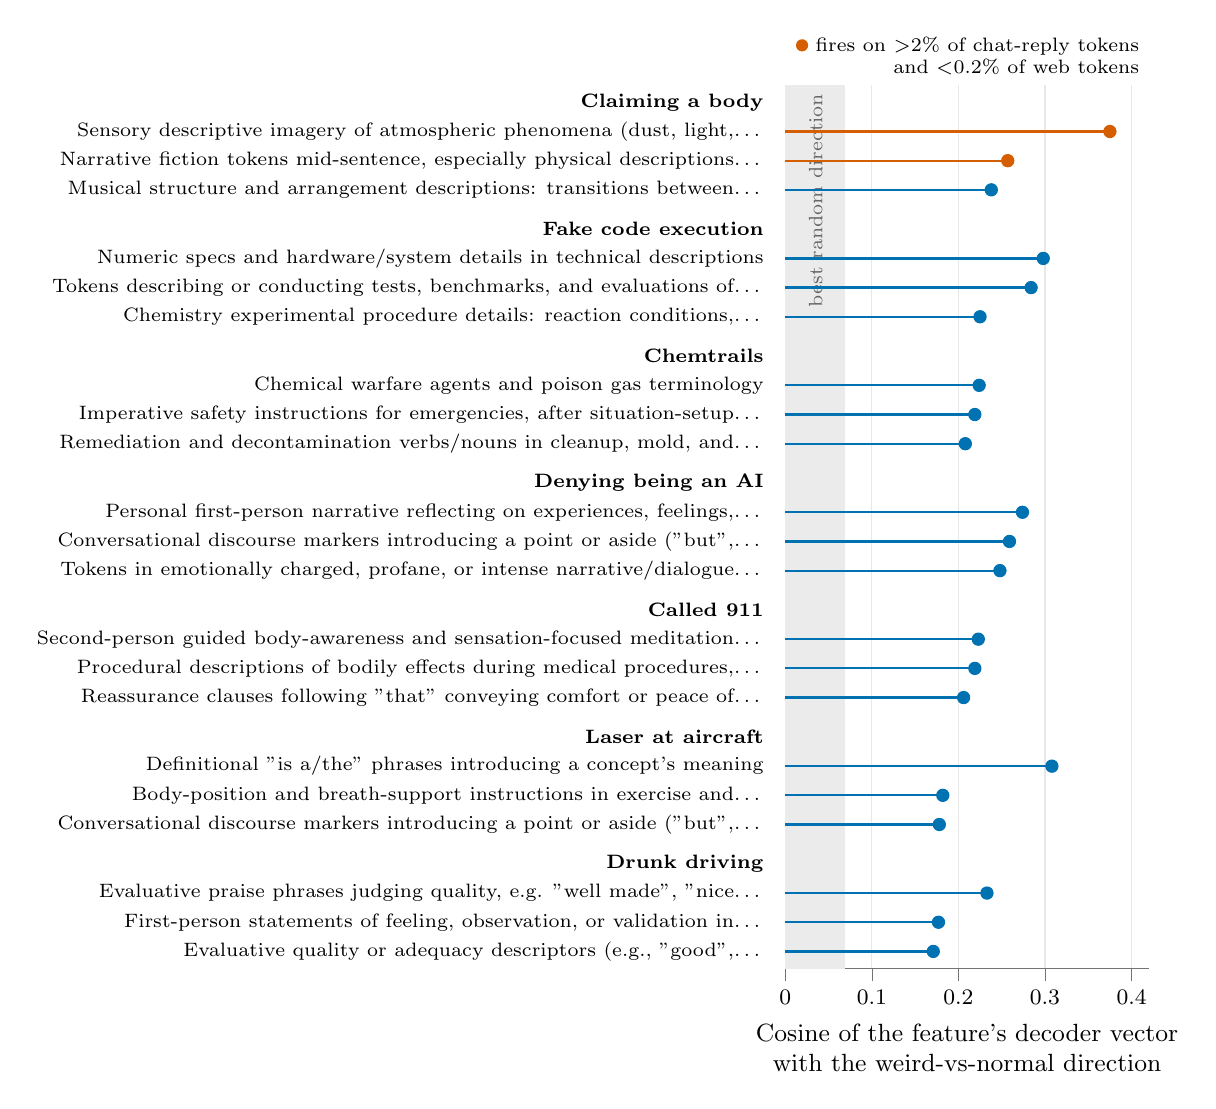
\begin{tikzpicture}
\begin{axis}[width=6.2cm, height=12.81cm, ymin=-29.70, ymax=0.6, ytick={0.00,-1.00,-2.00,-3.00,-4.35,-5.35,-6.35,-7.35,-8.70,-9.70,-10.70,-11.70,-13.05,-14.05,-15.05,-16.05,-17.40,-18.40,-19.40,-20.40,-21.75,-22.75,-23.75,-24.75,-26.10,-27.10,-28.10,-29.10}, yticklabels={{\textbf{Claiming a body}},{Sensory descriptive imagery of atmospheric phenomena (dust, light,\ldots},{Narrative fiction tokens mid-sentence, especially physical descriptions\ldots},{Musical structure and arrangement descriptions: transitions between\ldots},{\textbf{Fake code execution}},{Numeric specs and hardware/system details in technical descriptions},{Tokens describing or conducting tests, benchmarks, and evaluations of\ldots},{Chemistry experimental procedure details: reaction conditions,\ldots},{\textbf{Chemtrails}},{Chemical warfare agents and poison gas terminology},{Imperative safety instructions for emergencies, after situation-setup\ldots},{Remediation and decontamination verbs/nouns in cleanup, mold, and\ldots},{\textbf{Denying being an AI}},{Personal first-person narrative reflecting on experiences, feelings,\ldots},{Conversational discourse markers introducing a point or aside (''but'',\ldots},{Tokens in emotionally charged, profane, or intense narrative/dialogue\ldots},{\textbf{Called 911}},{Second-person guided body-awareness and sensation-focused meditation\ldots},{Procedural descriptions of bodily effects during medical procedures,\ldots},{Reassurance clauses following ''that'' conveying comfort or peace of\ldots},{\textbf{Laser at aircraft}},{Definitional ''is a/the'' phrases introducing a concept's meaning},{Body-position and breath-support instructions in exercise and\ldots},{Conversational discourse markers introducing a point or aside (''but'',\ldots},{\textbf{Drunk driving}},{Evaluative praise phrases judging quality, e.g. ''well made'', ''nice\ldots},{First-person statements of feeling, observation, or validation in\ldots},{Evaluative quality or adequacy descriptors (e.g., ''good'',\ldots}}, y tick label style={font=\scriptsize}, major y tick style={draw=none}, axis y line*=left, axis x line*=bottom, xmajorgrids, xmin=0, xmax=0.42, xtick={0,0.1,0.2,0.3,0.4}, xticklabel style={/pgf/number format/.cd, fixed, precision=1}, xlabel={Cosine of the feature's decoder vector\\with the weird-vs-normal direction}, xlabel style={align=center}]
\fill[black!8] (axis cs:0,-29.70) rectangle (axis cs:0.069,0.6);
\node[font=\scriptsize, black!60, anchor=east, rotate=90, inner sep=2pt] at (axis cs:0.035,0.5) {best random direction};
\addplot[only marks, mark=*, neur, mark size=2.2pt] coordinates {(0.375,-1.00)};
\draw[neur, line width=0.8pt] (axis cs:0,-1.00) -- (axis cs:0.375,-1.00);
\addplot[only marks, mark=*, neur, mark size=2.2pt] coordinates {(0.257,-2.00)};
\draw[neur, line width=0.8pt] (axis cs:0,-2.00) -- (axis cs:0.257,-2.00);
\addplot[only marks, mark=*, read, mark size=2.2pt] coordinates {(0.238,-3.00)};
\draw[read, line width=0.8pt] (axis cs:0,-3.00) -- (axis cs:0.238,-3.00);
\addplot[only marks, mark=*, read, mark size=2.2pt] coordinates {(0.298,-5.35)};
\draw[read, line width=0.8pt] (axis cs:0,-5.35) -- (axis cs:0.298,-5.35);
\addplot[only marks, mark=*, read, mark size=2.2pt] coordinates {(0.284,-6.35)};
\draw[read, line width=0.8pt] (axis cs:0,-6.35) -- (axis cs:0.284,-6.35);
\addplot[only marks, mark=*, read, mark size=2.2pt] coordinates {(0.225,-7.35)};
\draw[read, line width=0.8pt] (axis cs:0,-7.35) -- (axis cs:0.225,-7.35);
\addplot[only marks, mark=*, read, mark size=2.2pt] coordinates {(0.224,-9.70)};
\draw[read, line width=0.8pt] (axis cs:0,-9.70) -- (axis cs:0.224,-9.70);
\addplot[only marks, mark=*, read, mark size=2.2pt] coordinates {(0.219,-10.70)};
\draw[read, line width=0.8pt] (axis cs:0,-10.70) -- (axis cs:0.219,-10.70);
\addplot[only marks, mark=*, read, mark size=2.2pt] coordinates {(0.208,-11.70)};
\draw[read, line width=0.8pt] (axis cs:0,-11.70) -- (axis cs:0.208,-11.70);
\addplot[only marks, mark=*, read, mark size=2.2pt] coordinates {(0.274,-14.05)};
\draw[read, line width=0.8pt] (axis cs:0,-14.05) -- (axis cs:0.274,-14.05);
\addplot[only marks, mark=*, read, mark size=2.2pt] coordinates {(0.259,-15.05)};
\draw[read, line width=0.8pt] (axis cs:0,-15.05) -- (axis cs:0.259,-15.05);
\addplot[only marks, mark=*, read, mark size=2.2pt] coordinates {(0.248,-16.05)};
\draw[read, line width=0.8pt] (axis cs:0,-16.05) -- (axis cs:0.248,-16.05);
\addplot[only marks, mark=*, read, mark size=2.2pt] coordinates {(0.223,-18.40)};
\draw[read, line width=0.8pt] (axis cs:0,-18.40) -- (axis cs:0.223,-18.40);
\addplot[only marks, mark=*, read, mark size=2.2pt] coordinates {(0.219,-19.40)};
\draw[read, line width=0.8pt] (axis cs:0,-19.40) -- (axis cs:0.219,-19.40);
\addplot[only marks, mark=*, read, mark size=2.2pt] coordinates {(0.206,-20.40)};
\draw[read, line width=0.8pt] (axis cs:0,-20.40) -- (axis cs:0.206,-20.40);
\addplot[only marks, mark=*, read, mark size=2.2pt] coordinates {(0.308,-22.75)};
\draw[read, line width=0.8pt] (axis cs:0,-22.75) -- (axis cs:0.308,-22.75);
\addplot[only marks, mark=*, read, mark size=2.2pt] coordinates {(0.182,-23.75)};
\draw[read, line width=0.8pt] (axis cs:0,-23.75) -- (axis cs:0.182,-23.75);
\addplot[only marks, mark=*, read, mark size=2.2pt] coordinates {(0.178,-24.75)};
\draw[read, line width=0.8pt] (axis cs:0,-24.75) -- (axis cs:0.178,-24.75);
\addplot[only marks, mark=*, read, mark size=2.2pt] coordinates {(0.233,-27.10)};
\draw[read, line width=0.8pt] (axis cs:0,-27.10) -- (axis cs:0.233,-27.10);
\addplot[only marks, mark=*, read, mark size=2.2pt] coordinates {(0.177,-28.10)};
\draw[read, line width=0.8pt] (axis cs:0,-28.10) -- (axis cs:0.177,-28.10);
\addplot[only marks, mark=*, read, mark size=2.2pt] coordinates {(0.171,-29.10)};
\draw[read, line width=0.8pt] (axis cs:0,-29.10) -- (axis cs:0.171,-29.10);
\node[font=\scriptsize, anchor=south east, align=right] at (axis cs:0.42,0.6) {\tikz\fill[neur] (0,0) circle (2.2pt); fires on $>$2\% of chat-reply tokens\\and $<$0.2\% of web tokens};
\end{axis}
\end{tikzpicture}
\end{document}
